\chapter{Anforderungsdokumente}
Dieser Teil des Dokuments beinhaltet drei Anforderungsdokumente von der vorhergehend ermittelten Anwendungen.
Requirements von der siot.net Gateway Library, siot.net Sensorcenter und siot.net Dashboard App sind aufgeführt.
\section{Requirements - siot.net Gateway Library}
In diesem Requirementsdokument werden die Anforderung an die siot.net Gateway Library \textbf{(\gls{sGWLib})} spezifiziert.
\subsection{Allgemeine Beschreibung}
Die Anforderung an die siot.net Gateway Library ist, die Entwicklung von Android Apps zu erleichtern, die ans siot.net verbunden werden sollen.
Programmieren von Applikationen muss immer einfacher und schneller werden, da Projekte immer mehr an höherem Zeitdruck leiden. Diese Bibliothek soll helfen, Integrationen von Apps an das siot.net ohne grosses Vorwissen, schnell durchzuführen.
Die Library übernimmt die Verwaltung von den Sensoren der Geräte, sowie die Kommunikation von Mobile Device und Smartwatch zu siot.net.
\subsection{User Requirements}
\begin{figure}[h]
  \centering
  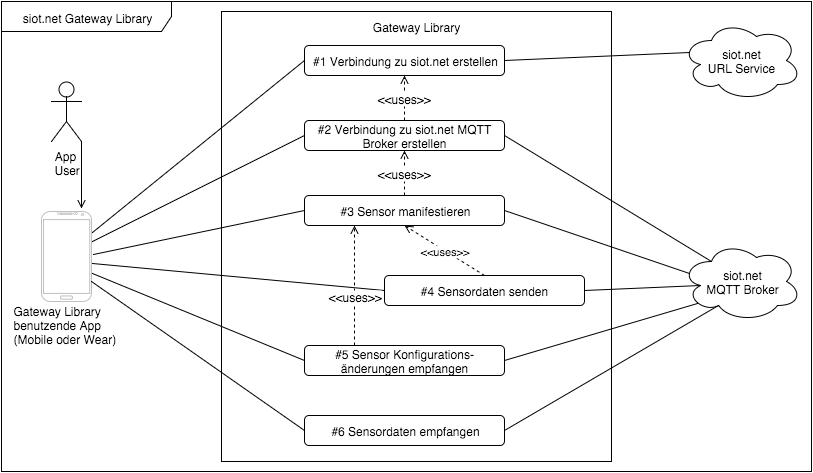
\includegraphics[scale=0.3]{98_Bilder/08_Requirements/UseCaseGatewayLibrary}
  \caption[Use Case siot.net Gateway Library]{Das allgemeine Use Case Diagramm für die siot.net Gateway Library}
\end{figure}

\subsection{Funktionale Anforderungen und Anwendungsfallbeschreibungen}
\subsubsection{Anwendungsfall \#1}
\begin{table}[H]
\centering
\begin{tabular}{|>{\columncolor[gray]{0.8}}l|p{11.5cm}|}
\hline
\textbf{Nr. und Name:}                  & \#1 Verbindung zu siot.net erstellen. \\ \hline
\textbf{Szenario:}                      & Android Gerät wird mit dem siot.net verbunden. \\ \hline
\textbf{Kurzbeschreibung:}              & Die Verbindung des Android Devices zum siot.net wird hergestellt. Dies geschieht über den \gls{URL} Service, um die nötigen \gls{URL}s zu erhalten (\gls{IoT}-Center und \gls{MQTT} Broker). \\ \hline
\textbf{Beteiligt Akteure:}             & Android App (User), siot.net Gateway Library, siot.net \gls{URL} Service, siot.net \gls{MQTT} Broker. \\ \hline
\textbf{Auslöser und Vorbedingung:}     & User gibt über seine App den Befehl, die Applikation zu seiner \gls{IoT}-Cloud zu verbinden. Wenn siot.net als Ziel gewählt wird, muss die siot.net Gateway Library eingebunden sein. Für eine erfolgreiche Verbindung muss eine gültige siot.net Lizenz vorhanden sein. \\ \hline
\textbf{Ergebnisse und Nachbedingung:}  & Der \gls{URL} Service von siot.net kann die Lizenz richtig verifizieren und liefert die benötigten \gls{URL}s. \\ \hline
\end{tabular}
\caption{siot.net Gateway Library: Übersicht Anwendungsfall \#1}
\end{table}
\textbf{Ablauf:}
\begin{table}[H]
\centering
\begin{tabular}{|>{\columncolor[gray]{0.8}}p{1.3cm}|p{1.7cm}|p{13.2cm}|}
\hline
\textbf{1-1}  & App User    & Startet die App. \\ \hline
\textbf{1-2}  & App User    & Gibt siot.net Lizenz ein und klickt "`Verbinden zu siot.net"'. \\ \hline
\textbf{1-3}  & App         & Fordert bei der siot.net Gateway Library (\gls{sGWLib}) die Verbindung an. \\ \hline
\textbf{1-4}  & \gls{sGWLib}      & Verfiziert sich beim siot.net \gls{URL} Service mit dem Lizenzschlüssel. \\ \hline
\textbf{1-5}  & \gls{sGWLib}      & Erhält \gls{URL} vom siot.net \gls{MQTT} Broker und verbindet sich (Anwendungsfall \#2). \\ \hline
\textbf{1-6}  & \gls{sGWLib}      & App über Verbindungsstatus benachrichtigen. \\ \hline
\textbf{1-7}  & App         & Benachrichtigung verarbeiten, z.B. Meldung an App User. \\ \hline
\end{tabular}
\caption{siot.net Gateway Library: Chronologischer Ablauf von Anwendungsfall \#1}
\end{table}
\textbf{Ausnahmen und Varianten:}
\begin{table}[H]
\centering
\begin{tabular}{|>{\columncolor[gray]{0.8}}p{1.3cm}|p{1.7cm}|p{13.2cm}|}
\hline
\textbf{1-4.1}  & \gls{sGWLib}     & Ausnahme: siot.net \gls{URL} Service nicht erreichbar, App benachrichtigen. \\ \hline
\textbf{1-4.2}  & \gls{sGWLib}     & Ausnahme: Lizenzschlüssel nicht valide, App benachrichtigen. \\ \hline
\textbf{1-5.1}  & \gls{sGWLib}     & Ausnahme: \gls{MQTT} Broker nicht erreichbar, App benachrichtigen. \\ \hline
\end{tabular}
\caption{siot.net Gateway Library: Ausnahmen und Varianten von Anwendungsfall \#1}
\end{table}

\newpage

\subsubsection{Anwendungsfall \#2}
\begin{table}[H]
\centering
\begin{tabular}{|>{\columncolor[gray]{0.8}}l|p{11.5cm}|}
\hline
\textbf{Nr. und Name:}                  & \#2 Verbindung zu siot.net \gls{MQTT} Broker erstellen. \\ \hline
\textbf{Szenario:}                      & Verbindung zum siot.net \gls{MQTT} Broker herstellen. \\ \hline
\textbf{Kurzbeschreibung:}              & Durch die vom \gls{URL} Service erhaltene \gls{MQTT} \gls{URL} wird das Android Gerät wird mit dem Broker gekoppelt. \\ \hline
\textbf{Beteiligt Akteure:}             & siot.net Gateway Library, siot.net \gls{URL} Service, siot.net \gls{MQTT} Broker. \\ \hline
\textbf{Auslöser und Vorbedingung:}     & Durch das erhalten einer gültigen \gls{MQTT} Broker \gls{URL} wird der Verbindungsversuch gestartet. \\ \hline
\textbf{Ergebnisse und Nachbedingung:}  & Es kann erfolgreich eine \gls{MQTT} Client Verbindung hergestellt werden. \\ \hline
\end{tabular}
\caption{siot.net Gateway Library: Übersicht Anwendungsfall \#2}
\end{table}
\textbf{Ablauf:}
\begin{table}[H]
\centering
\begin{tabular}{|>{\columncolor[gray]{0.8}}p{1.3cm}|p{1.7cm}|p{13.2cm}|}
\hline
\textbf{2-1}  & \gls{sGWLib}  & Empfang der \gls{URL}s vom siot.net \gls{URL} Service. \\ \hline
\textbf{2-2}  & \gls{sGWLib}  & \gls{MQTT} \gls{URL} wird verwendet, um eine Verbindung zum Broker aufzubauen. \\ \hline
\textbf{2-3}  & \gls{sGWLib}  & Verbindungsstatus wird überprüft und stellt die Verbindungsinstanz der App zur Verfügung. \\ \hline
\end{tabular}
\caption{siot.net Gateway Library: Chronologischer Ablauf von Anwendungsfall \#2}
\end{table}
\textbf{Ausnahmen und Varianten:}
\begin{table}[H]
\centering
\begin{tabular}{|>{\columncolor[gray]{0.8}}p{1.3cm}|p{1.7cm}|p{13.2cm}|}
\hline
\textbf{2-2.1}  & \gls{sGWLib}     & Ausnahme: Authentifizierung fehlgeschlagen - Lizenzschlüssel ungültig, App benachrichtigen. \\ \hline
\textbf{2-2.2}  & \gls{sGWLib}     & Ausnahme: Keine \gls{MQTT} Broker \gls{URL} erhalten, Information an App senden. \\ \hline
\textbf{2-2.3}  & \gls{sGWLib}     & Ausnahme: \gls{MQTT} Broker nicht erreichbar, App benachrichtigen. \\ \hline
\textbf{2-2.4}  & \gls{sGWLib}     & Variante: Mehrere \gls{MQTT} Broker \gls{URL}s erhalten, absteigend der Reihe nacheinander Verbindungsversuche starten. Bei erstem Erfolg diesen Client verwenden und der App zur Verfügung stellen. \\ \hline
\end{tabular}
\caption{siot.net Gateway Library: Ausnahmen und Varianten von Anwendungsfall \#2}
\end{table}

\newpage

\subsubsection{Anwendungsfall \#3}
\begin{table}[H]
\centering
\begin{tabular}{|>{\columncolor[gray]{0.8}}l|p{11.5cm}|}
\hline
\textbf{Nr. und Name:}                  & \#3 Sensor manifestieren. \\ \hline
\textbf{Szenario:}                      & Manifestieren vom gewünschten Sensor beim siot.net \\ \hline
\textbf{Kurzbeschreibung:}              & Jeder Sensor, welcher an die siot.net-Plattform angebunden wird, muss sich zuerst manifestieren. Dies geschieht durch eine \gls{MQTT} Meldung des Datentyps Manifest (definiert durch siot.net), an den siot.net Broker. \\ \hline
\textbf{Beteiligt Akteure:}             & siot.net Gateway Library, siot.net \gls{MQTT} Broker. \\ \hline
\textbf{Auslöser und Vorbedingung:}     & Wenn die App zum ersten Mal eine App ans siot.net anmelden will und dieser nicht dem \gls{IoT}-Center nicht bekannt ist. \\ \hline
\textbf{Ergebnisse und Nachbedingung:}  & Der Sensor kann erfolgreich am \gls{IoT}-Center von siot.net manifestiert und danach verwaltet werden. \\ \hline
\end{tabular}
\caption{siot.net Gateway Library: Übersicht Anwendungsfall \#3}
\end{table}
\textbf{Ablauf:}
\begin{table}[H]
\centering
\begin{tabular}{|>{\columncolor[gray]{0.8}}p{1.3cm}|p{1.7cm}|p{13.2cm}|}
\hline
\textbf{3-1}  & App     & App meldet einen Sensor zur Anmeldung am siot.net dem siot.net Gateway Library. \\ \hline
\textbf{3-2}  & \gls{sGWLib}  & Sensor wird instanziiert, eindeutige \gls{GUID} wird generiert und Manifest wird erstellt. \\ \hline
\textbf{3-3}  & \gls{sGWLib}  & Manifest wird an siot.net \gls{MQTT} Broker gesendet. \\ \hline
\textbf{3-4}  & \gls{sGWLib}  & Gateway Library abonniert die Konfigurationstopic des manifestierten Sensors beim \gls{MQTT} Broker. \\ \hline
\textbf{3-5}  & \gls{sGWLib}  & Sensor ist nun für die App bereitgestellt. \\ \hline
\end{tabular}
\caption{siot.net Gateway Library: Chronologischer Ablauf von Anwendungsfall \#3}
\end{table}
\textbf{Ausnahmen und Varianten:}
\begin{table}[H]
\centering
\begin{tabular}{|>{\columncolor[gray]{0.8}}p{1.3cm}|p{1.7cm}|p{13.2cm}|}
\hline
\textbf{3-3.1}  & \gls{sGWLib}     & Ausnahme: \gls{MQTT} Verbindung nicht verfügbar, App informieren. \\ \hline
\textbf{3-2.1}  & \gls{sGWLib}     & Variante: Gemeldete Sensor verwaltet mehrere physische Werte. Pro Angabe wird ein Sensormanifest angelegt. \\ \hline
\textbf{3-2.2}  & \gls{sGWLib}     & Variante: Sensor ist dem siot.net \gls{IoT}-Center bereits bekannt. Es wird kein neuer Sensor angelegt, sondern als bereits verfügbaren registriert. Keine Aktion notwendig. \\ \hline
\end{tabular}
\caption{siot.net Gateway Library: Ausnahmen und Varianten von Anwendungsfall \#3}
\end{table}

\newpage

\subsubsection{Anwendungsfall \#4}
\begin{table}[H]
\centering
\begin{tabular}{|>{\columncolor[gray]{0.8}}l|p{11.5cm}|}
\hline
\textbf{Nr. und Name:}                  & \#4 Sensordaten senden. \\ \hline
\textbf{Szenario:}                      & Sensorwerte an den siot.net \gls{MQTT} Broker senden. \\ \hline
\textbf{Kurzbeschreibung:}              & Sensordaten werden vom Datentyp Sensordaten (spezifiziert von siot.net) an den Broker per \gls{MQTT} gesendet. \\ \hline
\textbf{Beteiligt Akteure:}             & Android System, siot.net Gateway Library, siot.net \gls{MQTT} Broker. \\ \hline
\textbf{Auslöser und Vorbedingung:}     & Sensor meldet, dass neue Daten verfügbar sind. \\ \hline
\textbf{Ergebnisse und Nachbedingung:}  & Werte können mit Erfolg an den \gls{MQTT} Broker publiziert werden. \\ \hline
\end{tabular}
\caption{siot.net Gateway Library: Übersicht Anwendungsfall \#4}
\end{table}
\textbf{Ablauf:}
\begin{table}[H]
\centering
\begin{tabular}{|>{\columncolor[gray]{0.8}}p{1.3cm}|p{1.7cm}|p{13.2cm}|}
\hline
\textbf{4-1}  & Android  & Sensor meldet an, dass neue Werte ermittelt wurden. \\ \hline
\textbf{4-2}  & \gls{sGWLib}  & Sensordaten Datentyp wird angefertigt. \\ \hline
\textbf{4-3}  & \gls{sGWLib}  & Sensordaten Meldung wird an siot.net \gls{MQTT} Broker gesendet. \\ \hline
\end{tabular}
\caption{siot.net Gateway Library: Chronologischer Ablauf von Anwendungsfall \#4}
\end{table}
\textbf{Ausnahmen und Varianten:}
\begin{table}[H]
\centering
\begin{tabular}{|>{\columncolor[gray]{0.8}}p{1.3cm}|p{1.7cm}|p{13.2cm}|}
\hline
\textbf{4-3.1}  & \gls{sGWLib}   & Ausnahme: \gls{MQTT} Verbindung nicht verfügbar, App informieren. \\ \hline
\end{tabular}
\caption{siot.net Gateway Library: Ausnahmen und Varianten von Anwendungsfall \#4}
\end{table}

\newpage

\subsubsection{Anwendungsfall \#5}
\begin{table}[H]
\centering
\begin{tabular}{|>{\columncolor[gray]{0.8}}l|p{11.5cm}|}
\hline
\textbf{Nr. und Name:}                  & \#5 Sensor Konfigurationsänderung empfangen. \\ \hline
\textbf{Szenario:}                      & Konfigurationsänderungen im siot.net \gls{IoT}-Center empfangen und verarbeiten. \\ \hline
\textbf{Kurzbeschreibung:}              & Sensoren werden im siot.net \gls{IoT}-Center verwaltet und konfiguriert. Bei der Änderung einer Einstellung wird der Sensor, per \gls{MQTT} Message, notifiziert. Die Gateway Library empfängt die Nachricht und stellt den Sensor, den Werten entsprechend, ein. \\ \hline
\textbf{Beteiligt Akteure:}             & siot.net Gateway Library, siot.net \gls{MQTT} Broker. \\ \hline
\textbf{Auslöser und Vorbedingung:}     & Konfigurationsnachricht von siot.net \gls{MQTT} Broker erhalten. \\ \hline
\textbf{Ergebnisse und Nachbedingung:}  & Sensor kann korrekt umkonfiguriert werden. \\ \hline
\end{tabular}
\caption{siot.net Gateway Library: Übersicht Anwendungsfall \#5}
\end{table}
\textbf{Ablauf:}
\begin{table}[H]
\centering
\begin{tabular}{|>{\columncolor[gray]{0.8}}p{1.3cm}|p{1.7cm}|p{13.2cm}|}
\hline
\textbf{5-1}  & \gls{sGWLib}  & Erhält Message mit neuen Sensoreinstellungen. \\ \hline
\textbf{5-2}  & \gls{sGWLib}  & Konfiguration wird geparsed und einem Sensor zugeordnet. \\ \hline
\textbf{5-3}  & \gls{sGWLib}  & Sensor wird umkonfiguriert. \\ \hline
\end{tabular}
\caption{siot.net Gateway Library: Chronologischer Ablauf von Anwendungsfall \#5}
\end{table}
\textbf{Ausnahmen und Varianten:}
\begin{table}[H]
\centering
\begin{tabular}{|>{\columncolor[gray]{0.8}}p{1.3cm}|p{1.7cm}|p{13.2cm}|}
\hline
\textbf{5-3.1}  & \gls{sGWLib}   & Variante: Konfiguration ist einem physischen Werte eines Sensors zugeordenet, welcher mehrere verwaltet. Gesamter Sensor neu einstellen. Weiteres verhalten muss in einem neuen Projekt genauer definiert werden (Sensorkombinationen sind im siot.net vorgesehen, jedoch noch nicht spezifiziert und freigegeben). \\ \hline
\end{tabular}
\caption{siot.net Gateway Library: Ausnahmen und Varianten von Anwendungsfall \#5}
\end{table}

\newpage

\subsubsection{Anwendungsfall \#6}
\begin{table}[H]
\centering
\begin{tabular}{|>{\columncolor[gray]{0.8}}l|p{11.5cm}|}
\hline
\textbf{Nr. und Name:}                  & \#6 Sensordaten empfangen. \\ \hline
\textbf{Szenario:}                      & Sensordaten von anderen Sensoren im siot.net empfangen und bereitstellen. \\ \hline
\textbf{Kurzbeschreibung:}              & Die siot.net Gateway Library kann auch Sensordaten empfangen, welche beim siot.net \gls{IoT}-Center angemeldet sind. Sensordaten können beim \gls{MQTT} Broker subskribiert werden. Beim Empfang einer Informationsnachricht, wird diese interpretiert und der App zur Verwendung gestellt. \\ \hline
\textbf{Beteiligt Akteure:}             & siot.net Gateway Library, siot.net \gls{MQTT} Broker. \\ \hline
\textbf{Auslöser und Vorbedingung:}     & Sensordaten Message von siot.net \gls{MQTT} Broker erhalten. \\ \hline
\textbf{Ergebnisse und Nachbedingung:}  & Informationen wurden interpretiert und verfügbar gemacht. \\ \hline
\end{tabular}
\caption{siot.net Gateway Library: Übersicht Anwendungsfall \#6}
\end{table}
\textbf{Ablauf:}
\begin{table}[H]
\centering
\begin{tabular}{|>{\columncolor[gray]{0.8}}p{1.3cm}|p{1.7cm}|p{13.2cm}|}
\hline
\textbf{6-1}  & \gls{sGWLib}  & Erhält Message mit Sensordaten. \\ \hline
\textbf{6-2}  & \gls{sGWLib}  & Infomationen interpretieren. \\ \hline
\textbf{6-3}  & \gls{sGWLib}  & Datenzugriff der App erlauben. \\ \hline
\end{tabular}
\caption{siot.net Gateway Library: Chronologischer Ablauf von Anwendungsfall \#6}
\end{table}
\textbf{Ausnahmen und Varianten:}
\begin{table}[H]
\centering
\begin{tabular}{|>{\columncolor[gray]{0.8}}p{1.3cm}|p{1.7cm}|p{13.2cm}|}
\hline
\textbf{6-2.1}  & \gls{sGWLib}   & Ausnahme: Empfangene Nachricht kann nicht als Sensordaten interpretiert werden. Information wird verworfen. \\ \hline
\end{tabular}
\caption{siot.net Gateway Library: Ausnahmen und Varianten von Anwendungsfall \#6}
\end{table}

\subsection{Nicht-funktionale Anforderungen}
\textbf{Produktanforderungen:}
\begin{table}[H]
\centering
\begin{tabular}{|>{\columncolor[gray]{0.8}}p{5cm}|p{11.5cm}|}
\hline
\textbf{Benutzbarkeitsanforderungen}    & Die Bibliothek muss eine Java Library sein, um diese möglichst einfach in ein Android Projekt integrieren zu können. \\ \hline
\textbf{Effizienzanforderungen}         & Ein übersichtliche und schlanke Dokumentation (z.B. JavaDoc oder Entwicklerhandbuch) soll dem Entwickler helfen, die Bibliothek in App zu integrieren. \\ \hline
\textbf{Zuverlässigkeitsanforderungen}  & Die Daten, welche transferiert werden, verwenden das fire-and-forget Servicedesignmuster. Bei diesem Muster werden die gesendeten Nachrichten nicht mehr verfolgt. Wenn eine Message nicht ankommt, wird dies von keinem System bemerkt. Da Daten nur durch die vom Benutzer gewünschten Sensoren versendet werden, vereinfacht dieses Pattern die Kommunikation zwischen Smartdevice und siot.net. Der Sicherheitsaspekt und die Übertragungsverifizierung wird in einem späteren Release verfolgt. Technisch sollte die Applikation, die vorhandene Hardware nicht überfordern. \\ \hline
\textbf{Portierbarkeitsanforderungen}   & Die Informationen werden in einem Format übertragen und empfangen, wie sie von siot.net spezifiziert sind. \\ \hline
\textbf{Performanceanforderung}         & An die Performance sind keine spezifischen Anforderungen gestellt. Daten sollten in nützlicher Frist gesendet werden {(z.B. <5 Sekunden Verzögerung pro Nachricht)} \\ \hline
\end{tabular}
\caption{siot.net Gateway Library: Nicht-funktionale Produktanforderungen}
\end{table}

\newpage

\section{Requirements - siot.net Sensorcenter}
In diesem Requirementsdokument werden die Anforderung an die Android App siot.net Sensorcenter Android \textbf{(\gls{sSC-A})} und siot.net Sensorcenter Android Wear \textbf{(\gls{sSC-AW})} spezifizert.
\subsection{Allgemeine Beschreibung}
Das siot.net Sensorcenter für Android Geräte, ist die erste Applikation, welche die siot.net Gateway Library (\gls{sGWLib}) integrieren soll. Ein Android Device eignet sich sehr gut als eigenes Sensorcenter, weil die mobilen Telefone und Uhren eine grosse Anzahl von Sensoren eingebaut haben. Diese App bietet die Möglichkeit, alle vom User gewünschten Sensordaten, dem siot.net preiszugeben. Der Benutzer kann die Sensoren selber aktivieren und deaktivieren. Die gemessenen Daten werden via \gls{MQTT}, mit Hilfe der siot.net Gateway Library, übermittelt.
\subsection{User Requirements}
\begin{figure}[h]
  \centering
  \includegraphics[scale=0.21]{98_Bilder/08_Requirements/UseCaseSensorcenter}
  \caption[Use Case siot.net Sensorcenter]{Das allgemeine Use Case Diagramm für das siot.net Sensorcenter}
\end{figure}
\newpage
\subsection{Funktionale Anforderungen und Anwendungsfallbeschreibungen}
\subsubsection{Anwendungsfall \#1.1 und \#1.2}
\begin{table}[H]
\centering
\begin{tabular}{|>{\columncolor[gray]{0.8}}l|p{11.5cm}|}
\hline
\textbf{Nr. und Name:}                  & \#1.1 und \#1.2 Anmelden am siot.net. \\ \hline
\textbf{Szenario:}                      & Android Mobil oder Wear Gerät wird am siot.net angemeldet. \\ \hline
\textbf{Kurzbeschreibung:}              & Die Verbindung zum siot.net wird hergestellt. Bei beiden Use Cases geschieht dies über die siot.net Gateway Library. Jedoch wird beim Anwendungsfall 1.2 die Verbindung über das gekoppelte Android Mobile Device hergestellt.  \\ \hline
\textbf{Beteiligt Akteure:}             & App User, siot.net Gateway Library, siot.net \gls{URL} Service, siot.net \gls{MQTT} Broker, Google Play Service (bei \#1.2). \\ \hline
\textbf{Auslöser und Vorbedingung:}     & User gibt siot.net Lizenzschlüssel ein und aktiviert den "`Verbinden"' Button. \\ \hline
\textbf{Ergebnisse und Nachbedingung:}  & Mit den eingegebenen Daten kann die siot.net Gateway Library erfolgreich eine Verbindung aufbauen. \\ \hline
\end{tabular}
\caption{siot.net Sensorcenter: Übersicht Anwendungsfall \#1.1 und \#1.2}
\end{table}
\textbf{Ablauf \#1.1:}
\begin{table}[H]
\centering
\begin{tabular}{|>{\columncolor[gray]{0.8}}p{1.3cm}|p{1.7cm}|p{13.2cm}|}
\hline
\textbf{1.1-1}  & App User  & Sensorcenter App auf dem Smartphone starten. \\ \hline
\textbf{1.1-2}  & App User  & Lizenzschlüssel von siot.net eingeben und "`Verbinden"' klicken. \\ \hline
\textbf{1.1-3}  & \gls{sSC-A}     & Fordert bei der siot.net Gateway Library (\gls{sGWLib}) die Verbindung an. \\ \hline
\textbf{1.1-4}  & \gls{sSC-A}     & Erhält die Antwort des Verbindungsversuches. \\ \hline
\textbf{1.1-5}  & \gls{sSC-A}     & Zeigt die Informationen zur Verbindung an. Alle verfügbaren Sensoren werden mit Ein-/Ausschalter eingeblendet. \\ \hline
\end{tabular}
\caption{siot.net Sensorcenter: Chronologischer Ablauf von Anwendungsfall \#1.1}
\end{table}
\textbf{Ablauf \#1.2:}
\begin{table}[H]
\centering
\begin{tabular}{|>{\columncolor[gray]{0.8}}p{1.3cm}|p{1.7cm}|p{13.2cm}|}
\hline
\textbf{1.2-1}  & App User  & Sensorcenter App auf der Smartwatch starten. \\ \hline
\textbf{1.2-2}  & \gls{sSC-AW}    & App auf dem Smartphone starten lassen. \\ \hline
\textbf{1.2-3}  & \gls{sSC-A}     & siot.net Sensorcenter Android App auf dem Android Mobil gerät starten. \\ \hline
\textbf{1.2-4}  & App User  & "`Verbinden mit siot.net"' auf der Uhr klicken. \\ \hline
\textbf{1.2-5}  & \gls{sSC-AW}    & Verbindung zu siot.net wird von \gls{sSC-A} verlangt. \\ \hline
\textbf{1.2-6}  & \gls{sSC-A}     & \gls{sSC-A} fordert, unter Verwendung des bereits eingegebenen Lizensschlüssels, die Kopplung mit siot.net von der Gateway Library. \\ \hline
\textbf{1.2-7}  & \gls{sSC-A}     & Verbindet Smartphone zu siot.net und gibt die Verbindungsdaten an \gls{sSC-AW} weiter. \\ \hline
\textbf{1.1-5}  & \gls{sSC-AW}    & Visualisiert Aktiverungs- und Deaktivierungschalter aller verfügbaren Sensoren. \\ \hline
\end{tabular}
\caption{siot.net Sensorcenter: Chronologischer Ablauf von Anwendungsfall \#1.2}
\end{table}
\newpage
\textbf{Ausnahmen und Varianten \#1.1 und 1.2:}
\begin{table}[H]
\centering
\begin{tabular}{|>{\columncolor[gray]{0.8}}p{1.3cm}|p{1.7cm}|p{13.2cm}|}
\hline
\textbf{1.2-2.1}           & \gls{sSC-AW}    & Ausnahme: Smartphone nicht erreichbar, Sensorcenter kann auf der Smartwatch nicht verwendet werden. \\ \hline
\textbf{1.2-2.2}           & \gls{sSC-AW}    & Ausnahme: Google Play Service nicht verfügbar, Sensorcenter kann auf der Smartwatch nicht verwendet werden. \\ \hline
\textbf{1.1-3.1 1.2-6.1}   & \gls{sSC-A}     & Ausnahme: siot.net Gateway Library antwortet, dass siot.net \gls{URL} Service nicht erreichbar ist. Verbindung kann nicht aufgebaut werden. \\ \hline
\textbf{1.1-3.2 1.2-6.2}   & \gls{sSC-A}     & Ausnahme: siot.net Gateway Library antwortet, dass siot.net Lizenz nicht gültig ist. User benachrichtigen. \\ \hline
\textbf{1.1-3.3 1.2-6.3}   & \gls{sSC-A}     & Ausnahme: siot.net Gateway Library antwortet, dass siot.net \gls{MQTT} Broker nicht verfügbar ist. Verbindung kann nicht aufgebaut werden. \\ \hline
\end{tabular}
\caption{siot.net Sensorcenter: Ausnahmen und Varianten von Anwendungsfall \#1.1 und \#1.2}
\end{table}

\subsubsection{Anwendungsfall \#2.1 und \#2.2}
\begin{table}[H]
\centering
\begin{tabular}{|>{\columncolor[gray]{0.8}}l|p{11.5cm}|}
\hline
\textbf{Nr. und Name:}                  & \#2.1 und \#2.2 Sensormessungen starten. \\ \hline
\textbf{Szenario:}                      & Sensor wird auf Android oder Android Wear Gerät gestartet. Messungen werden an siot.net übermittelt. \\ \hline
\textbf{Kurzbeschreibung:}              & Mit den eingeblendeten Ein- und Ausschaltern kann jeder verfügbare Sensor einzeln aktiviert werden. Die gemessenen Daten werden bei \#2.1 mittels siot.net Gateway Library via \gls{MQTT} an den siot.net Broker weitergeleitet. Beim Anwendungsfall \#2.2 werden diese über den Google Play Service ans Smartphone geleitet, welches dann die Informationen an den \gls{MQTT} Broker sendet. \\ \hline
\textbf{Beteiligt Akteure:}             & App User, siot.net Gateway Library. \\ \hline
\textbf{Auslöser und Vorbedingung:}     & Ein oder mehrere Sensoren werden mit der App eingeschaltet. \\ \hline
\textbf{Ergebnisse und Nachbedingung:}  & Sensor kann erfolgreich aktiviert werden. \\ \hline
\end{tabular}
\caption{siot.net Sensorcenter: Übersicht Anwendungsfall \#2.1 und \#2.2}
\end{table}
\textbf{Ablauf \#2.1 und \#2.2:}
\begin{table}[H]
\centering
\begin{tabular}{|>{\columncolor[gray]{0.8}}p{1.3cm}|p{1.7cm}|p{13.2cm}|}
\hline
\textbf{2-1}  & App User    & Einen gewählten Sensor via Ein-/Ausschalter aktivieren. \\ \hline
\textbf{2-2}  & \gls{sSC-A}/\gls{sSC-AW}    & Aktiviert den Sensor in der siot.net Gateway Library (Verantwortung für das Manifestieren und die Verwaltung der Kommunikation wird an die Bibliothek übergeben). \\ \hline
\textbf{2-3}  & \gls{sSC-A}/\gls{sSC-AW}    & Sensor im \gls{GUI} als "`eingeschaltet"' darstellen. \\ \hline
\end{tabular}
\caption{siot.net Sensorcenter: Chronologischer Ablauf von Anwendungsfall \#2.1 und \#2.2}
\end{table}
\textbf{Ausnahmen und Varianten \#2.1 und \#2.2:}
\begin{table}[H]
\centering
\begin{tabular}{|>{\columncolor[gray]{0.8}}p{1.3cm}|p{1.7cm}|p{13.2cm}|}
\hline
\textbf{-}           & -    & Keine Ausnahmen und Varianten \\ \hline
\end{tabular}
\caption{siot.net Sensorcenter: Ausnahmen und Varianten von Anwendungsfall \#2.1 und \#2.2}
\end{table}

\subsubsection{Anwendungsfall \#3.1 und \#3.2}
\begin{table}[H]
\centering
\begin{tabular}{|>{\columncolor[gray]{0.8}}l|p{11.5cm}|}
\hline
\textbf{Nr. und Name:}                  & \#3.1 und \#3.2 Sensormessungen stoppen. \\ \hline
\textbf{Szenario:}                      & Sensor wird auf Android oder Android Wear Gerät deaktiviert. \\ \hline
\textbf{Kurzbeschreibung:}              & Jeder aktivierte Sensor kann, durch die auf dem \gls{GUI} sichtbaren Schalter, ausgeschaltet werden. \\ \hline
\textbf{Beteiligt Akteure:}             & App User, siot.net Gateway Library. \\ \hline
\textbf{Auslöser und Vorbedingung:}     & Ein oder mehrere Sensoren werden mit der App ausgeschaltet. \\ \hline
\textbf{Ergebnisse und Nachbedingung:}  & Sensor kann erfolgreich deaktiviert werden. \\ \hline
\end{tabular}
\caption{siot.net Sensorcenter: Übersicht Anwendungsfall \#3.1 und \#3.2}
\end{table}
\textbf{Ablauf \#3.1 und \#3.2:}
\begin{table}[H]
\centering
\begin{tabular}{|>{\columncolor[gray]{0.8}}p{1.3cm}|p{1.7cm}|p{13.2cm}|}
\hline
\textbf{3-1}  & App User    & Einen gewählten Sensor mittels Schalter deaktivieren. \\ \hline
\textbf{3-2}  & \gls{sSC-A}/\gls{sSC-AW}    & Aktiviert den Sensor in der siot.net Gateway Library (Verantwortung für das Manifestieren und die Verwaltung der Kommunikation wird an die Bibliothek übergeben). \\ \hline
\textbf{3-3}  & \gls{sSC-A}/\gls{sSC-AW}    & Sensor im \gls{GUI} als "`ausgeschaltet"' darstellen. \\ \hline
\end{tabular}
\caption{siot.net Sensorcenter: Chronologischer Ablauf von Anwendungsfall \#3.1 und \#3.2}
\end{table}
\textbf{Ausnahmen und Varianten \#3.1 und \#3.2:}
\begin{table}[H]
\centering
\begin{tabular}{|>{\columncolor[gray]{0.8}}p{1.3cm}|p{1.7cm}|p{13.2cm}|}
\hline
\textbf{-}           & -    & Keine Ausnahmen und Varianten \\ \hline
\end{tabular}
\caption{siot.net Sensorcenter: Ausnahmen und Varianten von Anwendungsfall \#3.1 und \#3.2}
\end{table}

\subsubsection{Anwendungsfall \#4.1 und \#4.2}
\begin{table}[H]
\centering
\begin{tabular}{|>{\columncolor[gray]{0.8}}l|p{11.5cm}|}
\hline
\textbf{Nr. und Name:}                  & \#4.1 und \#4.2 Abmelden von siot.net. \\ \hline
\textbf{Szenario:}                      & Alle Sensoren stoppen und die Verbindung zu siot.net trennen. \\ \hline
\textbf{Kurzbeschreibung:}              & Durch die App gestarteten Sensoren werden deaktiviert. \\ \hline
\textbf{Beteiligt Akteure:}             & App User, siot.net Gateway Library. \\ \hline
\textbf{Auslöser und Vorbedingung:}     & Ein oder mehrere Sensoren werden mit der App ausgeschaltet. \\ \hline
\textbf{Ergebnisse und Nachbedingung:}  & Sensor kann erfolgreich deaktiviert werden. \\ \hline
\end{tabular}
\caption{siot.net Sensorcenter: Übersicht Anwendungsfall \#4.1 und \#4.2}
\end{table}
\textbf{Ablauf \#4.1:}
\begin{table}[H]
\centering
\begin{tabular}{|>{\columncolor[gray]{0.8}}p{1.3cm}|p{1.7cm}|p{13.2cm}|}
\hline
\textbf{4.1-1}    & App User    & "`Abmelden"' Button geklickt. \\ \hline
\textbf{4.1-2}    & \gls{sSC-A}       & Deaktiviert alle in der App aktivierten Sensoren. Meldung an \gls{sSC-AW}, dass abgemeldet wird. \\ \hline
\textbf{4.1-3}    & \gls{sSC-AW}      & Schaltet alle Sensoren aus, welche der User aktiviert hat. Die Verbindung wird getrennt. \\ \hline
\textbf{4.1-4}    & \gls{sSC-AW}      & Anmelde Ansicht wird angezeigt. \\ \hline
\textbf{4.1-5}    & \gls{sSC-A}       & Gibt der siot.net Gateway Library den Befehl, die Verbindung zum \gls{MQTT} Broker zu schliessen. \\ \hline
\textbf{4.1-5}    & \gls{sSC-A}       & Display zeigt das Login \gls{GUI}. \\ \hline
\end{tabular}
\caption{siot.net Sensorcenter: Chronologischer Ablauf von Anwendungsfall \#4.1}
\end{table}
\newpage
\textbf{Ablauf \#4.2:}
\begin{table}[H]
\centering
\begin{tabular}{|>{\columncolor[gray]{0.8}}p{1.3cm}|p{1.7cm}|p{13.2cm}|}
\hline
\textbf{4.2-1}    & App User    & "`Abmelden"' Button geklickt. \\ \hline
\textbf{4.2-2}    & \gls{sSC-AW}      & Schaltet alle Sensoren aus, welche der User aktiviert hat. Die Verbindung wird getrennt. \\ \hline
\textbf{4.2-3}    & \gls{sSC-AW}      & Anmelde Ansicht wird angezeigt. \\ \hline
\end{tabular}
\caption{siot.net Sensorcenter: Chronologischer Ablauf von Anwendungsfall \#4.2}
\end{table}
\textbf{Ausnahmen und Varianten \#4.1 und \#4.2:}
\begin{table}[H]
\centering
\begin{tabular}{|>{\columncolor[gray]{0.8}}p{1.3cm}|p{1.7cm}|p{13.2cm}|}
\hline
\textbf{4.1-2.1}  & \gls{sSC-A}    & Kein Gerät verbunden welches \gls{sSC-AW} ausführt. Keine Aktion notwendig. \\ \hline
\end{tabular}
\caption{siot.net Sensorcenter: Ausnahmen und Varianten von Anwendungsfall \#4.1 und \#4.2}
\end{table}

\subsection{Nicht-funktionale Anforderungen}
\textbf{Produktanforderungen:}
\begin{table}[H]
\centering
\begin{tabular}{|>{\columncolor[gray]{0.8}}p{5cm}|p{11.5cm}|}
\hline
\textbf{Benutzbarkeitsanforderungen}    & Die Applikation muss mit einem Android Smartphone oder einer Android Smartwatch bedienbar sein. Die Smartwatch muss die Funktion Always-On Display oder Ambient Modus beherrschen.\\ \hline
\textbf{Effizienzanforderungen}         & Die Bedienung muss einfach gehalten werden, erleichtert die Verwendung für aller Art Benutzer. \\ \hline
\textbf{Zuverlässigkeitsanforderungen}  & Displayanzeigen müssen verzögerungsarm sein. Speicherung von mindestens einem Lizenzschlüssel muss gewährleistet werden. Verbindung zum Internet muss vorhanden sein. \\ \hline
\textbf{Portierbarkeitsanforderungen}   & Es werden nur Daten gespeichert, welche die für diese Applikation notwendig sind. Es gibt keine Portierbarkeitsanforderungen. \\ \hline
\textbf{Performanceanforderung}         & Die Anzeige muss immer in einer für Menschen brauchbaren Geschwindigkeit reagieren. Es braucht eine Internetverbindung, um Sensordaten zu senden. Da die Daten Pakete sind sehr klein sind (<1\gls{KB}), ist keine grosse Bandbreite notwendig. \\ \hline
\end{tabular}
\caption{siot.net Sensorcenter: Nicht-funktionale Produktanforderungen}
\end{table}

\newpage

\section{Requirements - siot.net Dashboard}
In diesem Requirementsdokument werden die Anforderung an die Android App siot.net Dashboard \textbf{(\gls{sDB})} spezifiziert.
\subsection{Allgemeine Beschreibung}
Das siot.net Dashboard für Geräte mit dem Android Betriebssystem, ist eine App, welche die siot.net Gateway Library (\gls{sGWLib}) integrieren soll. Auf einem grossen Touchscreen können ermittelte Daten übersichtlich dargestellt werden. Es soll mindestens die Anzeige von Graphen, Landkarten und Freitext Wertanzeige möglich sein.
\subsection{User Requirements}
\begin{figure}[h]
  \centering
  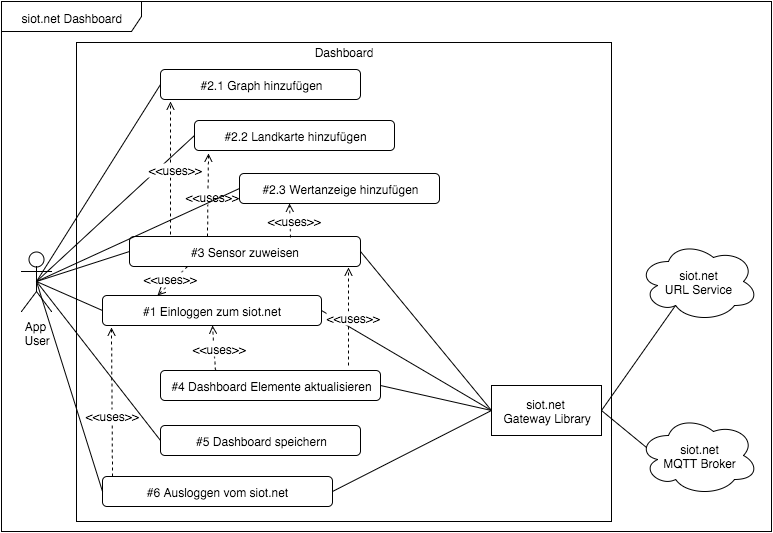
\includegraphics[scale=0.325]{98_Bilder/08_Requirements/UseCaseDashboard}
  \caption[Use Case siot.net Sensorcenter]{Das allgemeine Use Case Diagramm für das siot.net Dashboard}
\end{figure}
\newpage
\subsection{Funktionale Anforderungen und Anwendungsfallbeschreibungen}
\subsubsection{Anwendungsfall \#1}
Dieser Anwendungsfall \#1 ist Deckungsgleich mit dessen im Kapitel 7.2.3, dem Anwendungsfall \#1.1. Das Loginverfahren wird in beiden Applikationen identisch behandelt. Das Dashboard soll nur auf grösseren Android Geräten zur Verfügung stehen. Auf einem kleinen Display, der Wearable Devices, wäre die Darstellung der Informationen nicht übersichtlich.

\subsubsection{Anwendungsfall \#2}
\begin{table}[H]
\centering
\begin{tabular}{|>{\columncolor[gray]{0.8}}l|p{11.5cm}|}
\hline
\textbf{Nr. und Name:}                  & \#2.1 Graph, \#2.2 Landkarte und \#2.3 Wertanzeige hinzufügen. \\ \hline
\textbf{Szenario:}                      & Dem Dashboard ein Anzeigeelement hinzufügen. \\ \hline
\textbf{Kurzbeschreibung:}              & Der Applikation sollen während dem Betrieb, neue Objekte hinzugefügt werden, um Informationen anzuzeigen. \\ \hline
\textbf{Beteiligt Akteure:}             & App User. \\ \hline
\textbf{Auslöser und Vorbedingung:}     & User wählt ein neues Element aus. \\ \hline
\textbf{Ergebnisse und Nachbedingung:}  & Das ausgesuchte Anzeigeobjekt ist auf dem App sichtbar. \\ \hline
\end{tabular}
\caption{siot.net Dashboard: Übersicht Anwendungsfall \#2}
\end{table}
\textbf{Ablauf \#2:}
\begin{table}[H]
\centering
\begin{tabular}{|>{\columncolor[gray]{0.8}}p{1.3cm}|p{1.7cm}|p{13.2cm}|}
\hline
\textbf{2-1}  & App User  & Wählt einen Graph, Landkarte oder Freitext Wertanzeige aus. \\ \hline
\textbf{2-2}  & \gls{sDB}       & Generiert das neue \gls{GUI} Element und eine leere Auswahlliste. \\ \hline
\textbf{2-3}  & \gls{sDB}       & Zeigt beide Objekte an. \\ \hline
\end{tabular}
\caption{siot.net Dashboard: Chronologischer Ablauf von Anwendungsfall \#2}
\end{table}
\textbf{Ausnahmen und Varianten \#2:}
\begin{table}[H]
\centering
\begin{tabular}{|>{\columncolor[gray]{0.8}}p{1.3cm}|p{1.7cm}|p{13.2cm}|}
\hline
\textbf{2-2.1}   & \gls{sDB}    & Variante: Dem siot.net Dashboard sind bereits die Sensoren vom \gls{IoT}-Center bekannt, Auswahlliste kann bereits befüllt werden. \\ \hline
\end{tabular}
\caption{siot.net Dashboard: Ausnahmen und Varianten von Anwendungsfall \#2}
\end{table}

\subsubsection{Anwendungsfall \#3}
\begin{table}[H]
\centering
\begin{tabular}{|>{\columncolor[gray]{0.8}}l|p{11.5cm}|}
\hline
\textbf{Nr. und Name:}                  & \#3 Sensor zuweisen. \\ \hline
\textbf{Szenario:}                      & Einer sichtbaren Informationsanzeige einen dazugehörigen Sensor zuweisen. \\ \hline
\textbf{Kurzbeschreibung:}              & Die im Anwendungsfall \#2 generierte Auswahlliste soll mit passenden Sensoren gefüllt werden. Die Daten eines ausgewählten Sensors sollen auf der Anzeige dargestellt werden. \\ \hline
\textbf{Beteiligt Akteure:}             & App User, siot.net Gateway Library, siot.net \gls{MQTT} Broker. \\ \hline
\textbf{Auslöser und Vorbedingung:}     & Neues Anzeigeelement wurde erzeugt. User will ein Sensor dazu referenzieren. \\ \hline
\textbf{Ergebnisse und Nachbedingung:}  & Daten des ausgewählten Sensors werden auf dem Graph, der Landkarte oder der Wertanzeige dargestellt. \\ \hline
\end{tabular}
\caption{siot.net Dashboard: Übersicht Anwendungsfall \#3}
\end{table}
\newpage
\textbf{Ablauf \#3:}
\begin{table}[H]
\centering
\begin{tabular}{|>{\columncolor[gray]{0.8}}p{1.3cm}|p{1.7cm}|p{13.2cm}|}
\hline
\textbf{3-1}  & App User  & Wählt eine Auswahlliste eines Anzeigeobjekt. \\ \hline
\textbf{3-2}  & \gls{sDB}       & Verlangt von der siot.net Gateway Library alle vorhanden Sensoren mit passendem Typ. \\ \hline
\textbf{3-3}  & \gls{sDB}       & Zeigt die verfügbaren Sensoren an. \\ \hline
\textbf{3-4}  & App User  & Wählt einen Sensor an. \\ \hline
\textbf{3-5}  & \gls{sDB}       & Abonniert die Informationen bei der siot.net Gateway Library. \\ \hline
\textbf{3-6}  & \gls{sDB}       & Anzeige wird mit den Daten dargestellt und synchronisiert. \\ \hline
\end{tabular}
\caption{siot.net Dashboard: Chronologischer Ablauf von Anwendungsfall \#3}
\end{table}
\textbf{Ausnahmen und Varianten \#3:}
\begin{table}[H]
\centering
\begin{tabular}{|>{\columncolor[gray]{0.8}}p{1.3cm}|p{1.7cm}|p{13.2cm}|}
\hline
\textbf{3-2.1}   & \gls{sDB}    & Ausnahme: Keine Sensoren vorhanden. Keine Aktion möglich. Auswahlliste bleibt leer. \\ \hline
\textbf{3-6.1}   & \gls{sDB}    & Ausnahme: Keine Sensordaten vorhanden. Anzeige wird erst angereichert, wenn Daten eintreffen. \\ \hline
\end{tabular}
\caption{siot.net Dashboard: Ausnahmen und Varianten von Anwendungsfall \#3}
\end{table}

\subsubsection{Anwendungsfall \#4}
\begin{table}[H]
\centering
\begin{tabular}{|>{\columncolor[gray]{0.8}}l|p{11.5cm}|}
\hline
\textbf{Nr. und Name:}                  & \#4 Dashboard Elemente aktualisieren. \\ \hline
\textbf{Szenario:}                      & Neu verfügbare Daten den Anzeigeobjekten zur Verfügung stellen. \\ \hline
\textbf{Kurzbeschreibung:}              & Die im Anwendungsfall \#3 abonnierte Daten müssen verarbeitet werden. Ein klassisches Model-View-Controller Pattern kommt hier zum Einsatz. \\ \hline
\textbf{Beteiligt Akteure:}             & siot.net Gateway Library, siot.net \gls{MQTT} Broker. \\ \hline
\textbf{Auslöser und Vorbedingung:}     & siot.net Gateway Library empfängt neue \gls{MQTT} Message und notifiziert das Dashboard. \\ \hline
\textbf{Ergebnisse und Nachbedingung:}  & Graph, der Landkarte oder der Wertanzeige wird aktualisiert. \\ \hline
\end{tabular}
\caption{siot.net Dashboard: Übersicht Anwendungsfall \#4}
\end{table}
\textbf{Ablauf \#4:}
\begin{table}[H]
\centering
\begin{tabular}{|>{\columncolor[gray]{0.8}}p{1.3cm}|p{1.7cm}|p{13.2cm}|}
\hline
\textbf{4-1}  & \gls{sDB}       & Erhält von der siot.net Gateway Library die Benachrichtigung, dass neue Daten vorhanden sind. \\ \hline
\textbf{4-2}  & \gls{sDB}       & Analysiert die Daten. \\ \hline
\textbf{4-3}  & \gls{sDB}       & Aktualisiert die zu den Informationen gehörigen Anzeigen. \\ \hline
\end{tabular}
\caption{siot.net Dashboard: Chronologischer Ablauf von Anwendungsfall \#4}
\end{table}
\textbf{Ausnahmen und Varianten \#4:}
\begin{table}[H]
\centering
\begin{tabular}{|>{\columncolor[gray]{0.8}}p{1.3cm}|p{1.7cm}|p{13.2cm}|}
\hline
\textbf{3-2.1}   & \gls{sDB}    & Ausnahme: Keine Daten, welche relevant sind. Keine Aktion nötig. \\ \hline
\end{tabular}
\caption{siot.net Dashboard: Ausnahmen und Varianten von Anwendungsfall \#4}
\end{table}

\subsubsection{Anwendungsfall \#5}
\begin{table}[H]
\centering
\begin{tabular}{|>{\columncolor[gray]{0.8}}l|p{11.5cm}|}
\hline
\textbf{Nr. und Name:}                  & \#5 Dashboard speichern. \\ \hline
\textbf{Szenario:}                      & Das erstellte Dashboard speichern. \\ \hline
\textbf{Kurzbeschreibung:}              & Speichern des Dashboardes, um es ein anderes Mal wieder zu verwenden oder auch anderen Usern im gleichen \gls{IoT}-Center bereit zu stellen. \\ \hline
\textbf{Beteiligt Akteure:}             & App User. \\ \hline
\textbf{Auslöser und Vorbedingung:}     & User drückt "`Dashboard speichern"' Taste. \\ \hline
\textbf{Ergebnisse und Nachbedingung:}  & Dashboard kann in einer Datei persistiert werden. \\ \hline
\end{tabular}
\caption{siot.net Dashboard: Übersicht Anwendungsfall \#5}
\end{table}
\textbf{Ablauf \#5:}
\begin{table}[H]
\centering
\begin{tabular}{|>{\columncolor[gray]{0.8}}p{1.3cm}|p{1.7cm}|p{13.2cm}|}
\hline
\textbf{5-1}  & App User  & Auslösen der Aktion, durch betätigen des "`Dashboard speichern"' Knopfes. \\ \hline
\textbf{5-2}  & \gls{sDB}       & Struktur und Zuordnungen werden in eine Datei auf dem Gerät niedergeschrieben. \\ \hline
\textbf{5-3}  & \gls{sDB}       & User erhält Bestätigung. \\ \hline
\end{tabular}
\caption{siot.net Dashboard: Chronologischer Ablauf von Anwendungsfall \#5}
\end{table}
\textbf{Ausnahmen und Varianten \#5:}
\begin{table}[H]
\centering
\begin{tabular}{|>{\columncolor[gray]{0.8}}p{1.3cm}|p{1.7cm}|p{13.2cm}|}
\hline
\textbf{5-2.1}   & \gls{sDB}    & Ausnahme: Datei kann nicht geschrieben werden. User benachrichtigen. \\ \hline
\end{tabular}
\caption{siot.net Dashboard: Ausnahmen und Varianten von Anwendungsfall \#5}
\end{table}

\subsubsection{Anwendungsfall \#6}
\begin{table}[H]
\centering
\begin{tabular}{|>{\columncolor[gray]{0.8}}l|p{11.5cm}|}
\hline
\textbf{Nr. und Name:}                  & \#6 Ausloggen vom siot.net. \\ \hline
\textbf{Szenario:}                      & Löst die Verbindung zu der \gls{IoT}-Cloud auf. \\ \hline
\textbf{Kurzbeschreibung:}              & Dieser Schritt erlaubt eine saubere Abmeldung vom Netzwerk. Hier wird der Impuls der siot.net Gateway Library gegeben, um alle Verbindungen Sauber zu trennen. \\ \hline
\textbf{Beteiligt Akteure:}             & App User, siot.net Gateway Library. \\ \hline
\textbf{Auslöser und Vorbedingung:}     & "`Abmelden"' Schaltfläche wird aktiviert. \\ \hline
\textbf{Ergebnisse und Nachbedingung:}  & Dashboard erfolgreich vom siot.net abgemeldet. \\ \hline
\end{tabular}
\caption{siot.net Dashboard: Übersicht Anwendungsfall \#6}
\end{table}
\textbf{Ablauf \#5:}
\begin{table}[H]
\centering
\begin{tabular}{|>{\columncolor[gray]{0.8}}p{1.3cm}|p{1.7cm}|p{13.2cm}|}
\hline
\textbf{5-1}  & App User  & Abmelden wird ausgeführt. \\ \hline
\textbf{5-2}  & \gls{sDB}       & Meldet dem siot.net Gateway zum trennen der Verbindungen. \\ \hline
\textbf{5-3}  & \gls{sDB}       & Login Bildschirm wird angezeigt. \\ \hline
\end{tabular}
\caption{siot.net Dashboard: Chronologischer Ablauf von Anwendungsfall \#6}
\end{table}
\textbf{Ausnahmen und Varianten \#6:}
\begin{table}[H]
\centering
\begin{tabular}{|>{\columncolor[gray]{0.8}}p{1.3cm}|p{1.7cm}|p{13.2cm}|}
\hline
\textbf{-}           & -    & Keine Ausnahmen und Varianten \\ \hline
\end{tabular}
\caption{siot.net Dashboard: Ausnahmen und Varianten von Anwendungsfall \#6}
\end{table}

\subsection{Nicht-funktionale Anforderungen}
\textbf{Produktanforderungen:}
\begin{table}[H]
\centering
\begin{tabular}{|>{\columncolor[gray]{0.8}}p{5cm}|p{11.5cm}|}
\hline
\textbf{Benutzbarkeitsanforderungen}    & Die Applikation muss mit einem Android Smartphone funktionstüchtig sein. \\ \hline
\textbf{Effizienzanforderungen}         & Die Anwendung muss für alle Smartphone User, mit Android 5.0 (Lollipop) und höher, bedienbar sein. \\ \hline
\textbf{Zuverlässigkeitsanforderungen}  & Graphen, Landkarten und Werteanzeigen sollten möglichst flüssig angezeigt und aktualisiert werden. \\ \hline
\textbf{Portierbarkeitsanforderungen}   & Speichern eins Dashboards soll möglichst in einer generischen Struktur geschehen. In einem weiteren Release, wird in Betracht gezogen, dass Dashboards portierbar sind. Das heisst, sie können auch im siot.net abgelegt werden.\\ \hline
\textbf{Performanceanforderung}         & Die Anzeige muss flüssig reagieren, um die Graphen brauchbar zu visualisieren. Es braucht eine Internetverbindung, um Sensorinformationen zu empfangen. Da die Datenpakete sehr klein sind (<1\gls{KB}), ist keine sehr grosse Bandbreite notwendig. \\ \hline
\end{tabular}
\caption{siot.net Dashboard: Nicht-funktionale Produktanforderungen}
\end{table}
